\chapter{Book II: one picture to an opening}

\section{The shape of the record}

Book II is a stationer's journal with printed blue leaf numbers at the outer corner and a code, \q{C-1040 J}, at the foot of the cover. Its index, on leaf 1, is in pencil and is arranged not by title but by kind: \q{Oils p. 2 -- 33}, \q{77 -- 97 \struckq{(1939)} -- 1942.}, \q{French Oils -- p. 60 -- 63}, \q{Water colors p. 36 -- 60.}, \q{Julie photographs - list - p. 99.} (\lf{Book II}{1}{16974}). The volume that results is not chronological. Its front leaves hold the oils of October 1932 to 1942, in painting order; its middle holds the watercolours of 1932 to 1942 two to four to a leaf; and then, at leaf 60, it goes back thirty years, to the nine Paris oils of 1907--09, the early American oils of 1908--14, an inventory of what was left in Nyack, and the checklist of the Rehn show of January 1941, \q{Edward Hopper 1907--1914}, annotated over fifteen years. The book was begun in 1932, when the household moved from the rear studio to the front one at 3 Washington Square North, and the earlier work was written into it later, from memory and from the older books.

A leaf has the shape already described: the title and size in his hand; the record drawing, ruled into a box; the paint line; her description; the sale. The block migrates down the leaf as the years pass, and the transcription's advice is to read the head of each leaf rather than to assume. What does not migrate is the sale sentence, and it is worth quoting one entire because it is the atom of the whole archive: \q{May 13, 42 Chicago Art Institute - 3000 + return of Compartment C. 1000 - Com. 1/3 = 2000}, and below it, \q{Oct. 27, 42 Ada S. Garret Prize \$750} (\lf{Book II}{95}{17982}). That is the sale of Nighthawks. The picture cost three thousand dollars and a smaller canvas the museum had bought four years earlier and now handed back; the gallery took a third; the painter received two thousand, and five months later a prize.

\section{The descriptions}

What makes Book II unlike any other artist's ledger I know is the paragraph under the drawing. It begins, on the first leaves, as a note of light and colour, and it acquires almost at once the habit of naming the people in the picture and telling what they are doing. On the earliest leaves the voice is that of a painter looking at a landscape:

\begin{leafquote}
Late afternoon until dark, hills + house in silhouette against blue greeny sky with long strip of white clouds. Late Sept., tall grasses changing colors - pink in light. Hills roll for dear life! Field of tall grass in foregr. Entirely in light. Glorious! \hfill (Mrs. Scott's House, \lf{Book II}{2}{17332})
\end{leafquote}

\noindent Dauphinée House, on the same leaf: \q{Painted late in afternoon thru many changes of light til too dark to see. Peaceful before dark. House closed up + for sale. Built by a Capt. Kelly.} East Wind over Weehawken, with the painter in it: \q{Such cold raw weather, E. H. going over to Jersey to make sketches, could have caught pneumonia, but would go..} (\lf{Book II}{5}{17555}). Shakespeare at Dusk: \q{Mall, Central Park about 5 P.M. Nov. dusk with pink glow in sky back of trees. Foreground grey pavement, slightly warmed by glow in sky overhead (off stage).} and, at the end, a painter's self-criticism that is certainly not his: \q{Red, Electric sign showing thru foliage not well explained.} (\lf{Book II}{9}{18112}).

\q{Off stage} is her phrase and it recurs. She had been an actress with the Washington Square Players before she was his wife, and the pictures are described as scenes: what is lit from where, who stands where, what is happening beyond the edge. The Long Leg: \q{Boat white sailing into the wind. (Sun rear left off stage), light touching obliquely L. edges of sails, otherwise in shadow. Sails very taut, hard as marble in stiff breeze.} (\lf{Book II}{11}{17478}). The Sheridan Theatre: \q{Girl in bright red skirt, white jacket, dark fur collar, black hat + yellow curly hair (Mae West effect)} (\lf{Book II}{19}{17977}). New York Movie, which the leaf calls N.Y. Movie House, gets a lighting plot:

\begin{leafquote}
usher has yellow hair + flesh colored feet in black sandals. Dark blue uniform. Pewter grey + dull white on screen (snowy mountain tips) \ldots\ Light from 4 sources: bracket with 3 lights, right wall, light inside stair case R. light from lamps under side of boxes, L. + light from screen. \ldots\ Much darker than this sketch. Brightest point, girl's hair + glint on brass rail. \ldots\ Face resting on hand, hand light. L. hand holds end of flash light. \hfill (\lf{Book II}{27}{16621})
\end{leafquote}

\noindent \q{Much darker than this sketch}: the description corrects the drawing, hers correcting his, and the correction is about the one thing the drawing cannot carry, which is tone.

Then the anecdotes. Office at Night: \q{“Confidentatly Yours”. Room 1005.} and \q{Man in grey coat, blond hair. “Shirley” in blue dress, white collar, flesh stockings \ill\ pumps + black hair + plenty of lip stick. Figures stand out in space, not fastened to background.} (\lf{Book II}{79}{16494}). The Provincetown diary supplies the other half of that entry: on 22 February 1940 they took the canvas up to Rehn's, where there were \q{Attempts at christening; John Clancy suggesting: Cordially yours; Room 1566}. The title in the ledger, then, is a rejected joke of the dealer's, kept by her in quotation marks, and \q{Shirley} is a name she gave the secretary. Cape Cod Evening has a footnote: \q{* Was to have been called “Whipporwill.” Dog hears it. Woman a Finn + dour. Trees in phalanyx plantation, creeping up on one the dark. The whippoorwill in there out of sight.} and, further down, \q{Painted in S. Truro studio. Dog sat in poor \unc{Zerty's} car parked at Truro P.O.} (\lf{Book II}{31}{16755}). Gas: \q{Late twilight. Hanging sign “Mobiloil” + red horse lit from above, red pumps (3) with lamps lit \ldots\ Blond man in blue pants, white shirt, black vest tending pump - (son of Capt. Ed Staples burnt in train wreck returning from Cleveland Mus. show) \ldots\ (Notice light on sign, hauntingly familiar)} (\lf{Book II}{83}{18432}). The attendant, who has no face to speak of, is given a father, and the father is the sitter of an earlier picture, and that picture burnt in a railway accident recorded in Book I. The record books are a closed world and everything in them refers to everything else.

And Nighthawks, which she writes as two words:

\begin{leafquote}
Night + brilliant interior of cheap restaurant. Bright items; cheery wood counter + tops of surrounding stools; lights on metal tanks at rear right; brilliant streak of jade green tiles 3/4 across canvas - at base of glass of window. \ldots\ Very good looking blond boy in white (coat, cap) inside counter. Girl in red blouse, brown hair eating sandwich. Man night hawk (beek) in dark suit, steel grey hat, black band, blue shirt (clean) holding cigarette. Other figure dark sinister back - at left. \ldots\ Sign across top of \struckq{shop} dark - Phillies 5¢ Cigar, picture of cigar. \hfill (\lf{Book II}{95}{17982})
\end{leafquote}

\noindent \q{Man night hawk (beek)}: the title is explained as a nose. Nobody who has written about the picture since has had a better authority for what it was called and why, and the authority is a parenthesis in a ledger.

The transcription notices that the genre shifts. From leaf 45 the description \q{has stopped being an anecdote about who is in the picture and become a note of what color everything is}; on leaf 51 there is no description at all. The anecdotes belong to the oils of the 1930s and early 1940s, and to the figures in them; the watercolours of the Cape, which have no figures, get colour notes or nothing. Whatever the descriptions are, they are not a programme. They are what she thought worth saying about a picture on the day it left the studio, and on the days when the picture had people in it she gave the people names.

\begin{figure}[htbp]\centering
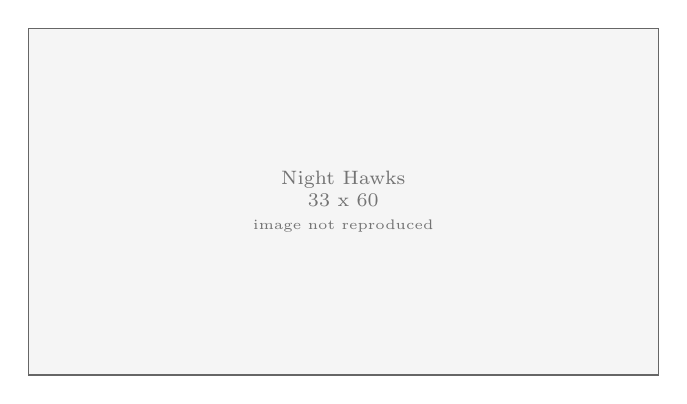
\begin{tikzpicture}
\draw[fill=black!4,draw=black!60,line width=0.5pt] (0,0) rectangle (8,4.4);
\node[align=center,text=black!55,font=\scriptsize] at (4,2.2) {Night Hawks\\33 x 60\\\tiny image not reproduced};
\end{tikzpicture}
\caption{\textbf{Night Hawks}, oil, finished 21 January 1942; catalogued as Nighthawks, 33 x 60 as the leaf writes it (Book II, leaf 95, ref 17982). Art Institute of Chicago, 1942.51: \url{https://www.artic.edu/artworks/111628}. Scale: sixty inches to eight centimetres. The frames are drawn to the proportions of the size in Edward Hopper's hand; the images are not reproduced here and can be seen at the museums' own pages. Drawn by Claude Fable~5.1, 13 September 2026, from the transcriptions and \texttt{works.json} (2026-09-13).}\label{fig:nighthawks}
\end{figure}


\section{Herself}

She is in the book as model, as painter and as owner. Jo Painting (\lf{Book II}{13}{16839}), a portrait of her, gets a description in the third person that is plainly a self-portrait in words: \q{Head against light. warm flesh tones against white background (painted on white canvas. greyish Blue wool dress with whitish crash collar, silver broach with green stone centre. Hair darkish brown + very bushy, just having been washed + waiting to dry thoroughly.} Its sale line reads \q{Given to wife, Jo N. Hopper as anniversary present | 1955}. Compartment C, Car 293: \q{A green picture (veridian + Cadmium deep) - green slightly olive. \ldots\ Girl with gold hair, flesh colored legs dressed in my purple wool jersey dress + black hat. \ldots\ On seat Reader's Digest in purple cover.} (\lf{Book II}{25}{18545}). The transcriber's note is exact: \q{the dress she puts on the girl is her own}. The Provincetown diary confirms that she posed, \q{by night light in big pokey hat \& hair down}, in March 1938, and again for Office at Night, \q{in a light skirt}, in February 1940. The women in the pictures of these years are Josephine Hopper in her own clothes, and the ledger says so in passing.

Her opinions are in it too. Cape Cod Afternoon, which won the Corcoran's first prize and two thousand dollars in 1937: \q{Looked good for nothing in dark Carnegie room, but glorious at Whitney Retrospective on W. 8th St.} (\lf{Book II}{17}{16656}); and on the same leaf, that the second prize went \q{to Guy Pène du Bois}, and that both winners were \q{dwellers of 3 Wash. Sq. N.} Blackwell's Island, sold to Russell Allen in 1929, gets a later pencil: \q{This a beautiful canvas but Russel Allen gone for the abstract in Boston so got rid of this canvas to son-in-law or nephew} (\lf{Book II}{35}{16536}). The politics of the house are on the watercolour leaves: \q{Returned to N.Y. early to go to Pittsburgh - jury} and \q{to register, then back from Cape early to N.Y.C. to vote against Roosevelt} (\lf{Book II}{55}{17435}); \q{Oct. 9, 40 brought back to N.Y. on hasty trip home to register for Willkie} (\lf{Book II}{83}{18432}). The year of the hurricane: \q{Watercolors - South Truro - 1933. Rained all summer.} (\lf{Book II}{39}{17049}); \q{1934 - The year we built the house, not much painting done.} (\lf{Book II}{42}{17766}).

\section{Paint}

Under nearly every oil, in the same words for thirty years, stands the formula. On the leaves of 1932 to 1936 it is \q{Zinc white, Rembrandt colors, poppy oil}; in 1937--38, \q{Belgian canvas, Rembrandt colors, lead white, linseed oil}; from 1939 the colourman changes to Winsor \& Newton, with Blockx beside it, and the whites and the oils begin to vary. The fullest is under The MacArthurs' Home, the portrait of Helen Hayes's house that the Provincetown diary says he \q{hates the imposed job} of painting: \q{Belgian smooth, double prime canvas, Blockx and Winsor \& Newton colors. poppy oil, Blockx Silver (lead) White. Sky of cerulean blue (Blockx) / 1 1/2 month painting.} (\lf{Book II}{77}{17681}). Nighthawks: \q{Blockx and Winsor \& Newton colors, W \& N. Zinc white, poppy oil. English linen, domestic priming.} She dates the Paris canvases by the paint: \q{Probably 1909 because white paint not altered. 1907 cheaper paint} (\lf{Book II}{61}{16607}). The change of colourman is dated to the week by the diary: on 18 May 1938, \q{E. wants to change over to Windsor Newton oils --- So I'm to inherit gold Rembrandt colors.} The Technique chapter takes this up; here it is enough to note that the formula is the one part of the leaf that is neither a measurement nor a report of an event, but her hand recording his practice.

\section{The money, and what came back}

The prices in Book II run from nine hundred dollars to eleven thousand. Cape Cod Afternoon went to the Carnegie for 3000 in 1938; New York Movie to Stephen Clark for 2500 in 1939; Gas to the Museum of Modern Art for 1800 in 1943; the Sheridan Theatre to Newark for 900 in 1940; Sun on Prospect Street to Edward G. Robinson, \q{someone in movie world named Robinson} as the diary has it, for 1000 the same year. The pictures that stayed longest sold highest: Dauphinée House, painted in October 1932, went to Huntington Hartford for 5000 in June 1956; Men, Women and Horses, of April 1939, to Leistner for 4500 in 1958; and Girlie Show, of April 1941, to Charles Stein in July 1961 for 11,000, \q{the highest price in Book II} as the transcriber notes (\lf{Book II}{89}{16635}). A canvas of 1913, Corner Saloon, was bought by the Museum of Modern Art out of the show of early work in January 1941, part paid in cash and part with \q{2 old water colors / given some years before by Mrs. John D. Rockefeller, Jr.} (\lf{Book II}{87}{18258}). Sailing, the first canvas sold, \q{Turned up + brought to Rehn Gal. ± 1951 + resold for \$1200. for owner} (\lf{Book II}{68}{16468}).

Museums took a discount over the dealer's third and the book records each: \q{Mus. discount 12\%} on East Wind over Weehawken to the Pennsylvania Academy; \q{10\% off of 2500} for Cape Cod Evening to the Encyclopaedia Britannica. The Whitney's purchase of the Circle Theatre for 1800 in 1936 was undone in 1950, when the museum returned it \q{for \$500 \ldots\ in exchange for 7 A.M.}, and the leaf follows the canvas to Stein at 2500 in 1951 (\textsc{Book II}, leaf 14 verso; \lf{Book II}{15}{18268}). Pictures came back: Capron House and Longnook Valley \q{Returned to Studio Nov. 12, '36}; Compartment C from Chicago in 1942, \q{Frame changed again. Art Inst. frame no good. They had changed original frame.} Pictures were given: Cape Cod Sunset and two Paris oils to her; Shacks at Pamet Head to Lloyd Goodrich; Route 14, Vermont to a Finnish relief auction; Dawn Before Gettysburg \q{presented to Arthuro Grassi! taken off to Italy}, with the dealer's assistant carrying the canvas down to the purser \q{after boat sailed} (\lf{Book II}{4}{18397}).

And there is the dealer's death. House at Dusk went to the Virginia Museum in 1953, and the leaf records what happened to the money: \q{Payment held up by illness of Frank Rehn beginning Sept. 53. Paid by Va. Mus. Early 1953. Death of Frank Rehn - Mar. 1956 - no provision in his will for payment of this sum.} (\lf{Book II}{6}{17606}). The date of Rehn's death is wrong here and wrong differently on the title page of Book III, and the transcription corrects neither; what the sentence records is that a museum's cheque, passed through a dying dealer's gallery, did not reach the painter until June 1956, and that the widow of the painter wrote it down.

\section{Arithmetic}

Five rows in the whole archive fail the check that the receipt equals the price less the commission, and two are in Book II: 2550 less a third written as 1660 on leaf 45, and 1250 less a third written as 850 on leaf 85 against 1275 to 850 on leaf 81, both cheques dated 29 December 1947. The transcription reports the disagreement and does not resolve it. Ninety of ninety-five checkable rows agree to the cent, which is a better rate than most published accounts of artists' incomes can claim, and it is the strongest evidence in the archive that the record was kept from the cheque and not from memory.
